\chapter{Method B --- Burst mode}
\label{sec:burst}

\begin{center}
\small
\begin{tabular}{@{}ll@{}}
\toprule
Notebook cell & Step 4B (analysis: Step 5B) \\
Code path & \co{prog.acquire(per_rep=True, reset_tproc=True)} \\
One call returns & \emph{every} rep as its own sample: \co{reps} samples \\
Measured rate & \textbf{4167\,Hz in-burst}, \textbf{3089\,Hz net} \\
Rate limited by & the FPGA cadence; the host cost is amortised over the burst \\
Duty cycle & \textbf{74.1\%} \\
Measured floor & \textbf{38\,\etaunit} --- best of the three \\
Open defects & \Open{} \textbf{49.9\% of bursts are replays} (\S\ref{sec:replay}) \\
\bottomrule
\end{tabular}
\end{center}

\section{Mechanics}

The FPGA program is identical to Method A's. The only change is that
\co{analyze_results(per_rep=True)} \emph{keeps} the rep axis: the second division
in Eq.~\ref{eq:divisions} is skipped, and the call returns a
$(\text{reps}\times n_\text{freqs})$ array. Every row is an independent time
sample spaced by $t_\text{rep}$.

The $\sim$11\,ms host chain is therefore paid once per \emph{burst} of 500 samples
instead of once per sample --- a 500$\times$ amortisation, which is where the rate
comes from.

\paragraph{The structural difference from Method A.} Here the FPGA time and the
host time \emph{do} add. Stage 6 of the chain (\S\ref{sec:rpc}) cannot return
until the tProc has finished all 500 reps, which takes \SI{120}{\milli\second} ---
far longer than the rest of the chain. The mode is genuinely FPGA-bound, which is
exactly what Method A is not.

\section{Timing budget, component by component}
\label{sec:burstbudget}

\subsection*{Operating point: $\tau=\SI{120}{\micro\second}$, 500 reps per burst (2026-08-14)}

\begin{center}
\small
\begin{tabular}{@{}lrrl@{}}
\toprule
\hd{Component} & \hd{Time per burst} & \hd{Share} & \hd{How obtained} \\
\midrule
\multicolumn{4}{@{}l}{\emph{Productive time}} \\
ADC integration: $500\times\SI{240}{\micro\second}$
  & \textbf{\SI{120.000}{\milli\second}} & 81.7\% & exact, Eq.~\ref{eq:recover} \\
\midrule
\multicolumn{4}{@{}l}{\emph{Overhead, per real burst}} \\
Host RPC chain (adds here)
  & \SI{14.697}{\milli\second} & 10.0\% & measured wall $-$ exact FPGA \\
\co{acquire()} total, real burst
  & \SI{134.697}{\milli\second} & 91.7\% & median of \co{acq_seconds}, real batches \\
\quad p05 / p95
  & 118.0 / \SI{136.3}{\milli\second} & & spread is host jitter \\
\midrule
\multicolumn{4}{@{}l}{\emph{Pure waste --- the open defect}} \\
Stale replay acquire
  & \SI{12.533}{\milli\second} & 8.5\% & $\times$185 batches \\
\quad total run time wasted
  & \textbf{\SI{2.32}{\second}} of \SI{30.11}{\second} & 7.7\% & produces no usable data \\
\midrule
\multicolumn{4}{@{}l}{\emph{Result}} \\
Total per usable sample
  & \textbf{\SI{0.324}{\milli\second}} & & \SI{30.11}{\second} / 92\,814 samples \\
Net rate & \textbf{3089\,Hz} & & \\
In-burst rate & \textbf{4167\,Hz} & & $1/t_\text{rep}$, exact \\
Duty cycle & \textbf{74.1\%} & & 22.32\,s of FPGA in 30.11\,s \\
\bottomrule
\end{tabular}
\end{center}

\begin{keybox}[Where the 26\% of non-productive time goes]
\begin{center}
\small
\begin{tabular}{@{}lrr@{}}
\toprule
\hd{Where the \SI{30.11}{\second} run went} & \hd{Time} & \hd{Share} \\
\midrule
ADC integration (productive)      & \SI{22.32}{\second} & \textbf{74.1\%} \\
Host chain, 186 real bursts       & \SI{2.73}{\second}  & 9.1\% \\
Stale replay acquires (waste)     & \SI{2.32}{\second}  & 7.7\% \\
Flushes, row-0 drops, residual    & \SI{2.74}{\second}  & 9.1\% \\
\bottomrule
\end{tabular}
\end{center}
Fixing the replay defect would recover the 7.7\% directly and would also remove
the wasted host chain on those calls --- roughly a 15\% rate gain, taking the net
rate from 3089\,Hz toward $\sim$3600\,Hz.
\end{keybox}

\subsection*{Operating point: $\tau=\SI{213}{\micro\second}$, 500 reps per burst (2026-08-06)}

\begin{center}
\small
\begin{tabular}{@{}lrrl@{}}
\toprule
\hd{Component} & \hd{Time per burst} & \hd{Share} & \hd{Note} \\
\midrule
ADC integration: $500\times\SI{426}{\micro\second}$ & \SI{213.001}{\milli\second} & 100.3\% & exact \\
Host RPC chain & $<$\SI{2.13}{\milli\second} & $<$1\% & below the resolution of timing a 213\,ms call \\
\co{acquire()} total, real burst & \SI{212.267}{\milli\second} & 100\% & measured \\
Stale replay acquire & \SI{12.648}{\milli\second} & 6.0\% & $\times$106 batches = \SI{1.34}{\second} wasted \\
Total per usable sample & \SI{0.514}{\milli\second} & & \\
Net rate & 1946\,Hz & & \\
In-burst rate & 2347\,Hz & & \\
Duty cycle & 82.9\% & & \\
\bottomrule
\end{tabular}
\end{center}

Note that the host share is a \emph{smaller} fraction here because the FPGA run is
longer --- the amortisation improves with burst length. That is the argument for
large \co{BURST_REPS}, bounded only by how long a gap in the time series is
acceptable and by the accumulated-buffer size.

\subsection{Rate against burst length}

With host chain $H\approx\SI{14.7}{\milli\second}$ and stale overhead
$S\approx\SI{12.5}{\milli\second}$ per real burst, the net rate is
\begin{equation}
f_\text{net} \;=\; \frac{N}{N\,t_\text{rep} + H + S}
\end{equation}
which at $\tau=\SI{120}{\micro\second}$ gives:

\begin{center}
\small
\begin{tabular}{@{}rrrr@{}}
\toprule
\hd{\co{BURST_REPS}} & \hd{FPGA per burst} & \hd{Net rate} & \hd{Duty cycle} \\
\midrule
100  & \SI{24.0}{\milli\second}  & 1961\,Hz & 47\% \\
250  & \SI{60.0}{\milli\second}  & 2874\,Hz & 69\% \\
\textbf{500}  & \textbf{\SI{120.0}{\milli\second}} & \textbf{3413\,Hz} & \textbf{82\%} \\
1000 & \SI{240.0}{\milli\second} & 3771\,Hz & 90\% \\
2000 & \SI{480.0}{\milli\second} & 3963\,Hz & 95\% \\
\bottomrule
\end{tabular}
\end{center}

(The 500-rep row predicts 3413\,Hz against 3089\,Hz measured; the difference is the
CSV flushes and the dropped row-0 samples.) The returns flatten past $\sim$1000
reps, and the gaps grow: a 2000-rep burst leaves a \SI{27}{\milli\second} hole in
the time series every \SI{480}{\milli\second}.

\section{Three artefacts, and what each one is}
\label{sec:burstartefacts}

The 2026-08-06 \file{Burst Mode.png} showed four visually distinct problems. All
four are now explained, and three are fixed.

\begin{center}
\small
\begin{tabular}{@{}p{3.8cm}p{7.6cm}p{3.0cm}@{}}
\toprule
\hd{What you see} & \hd{What it is} & \hd{Status} \\
\midrule
Large spike, strictly every $\sim$0.45\,s &
  Row 0 of each \emph{stale} batch: \textbf{+1908\,kHz $\approx$ +68\,\si{\micro\tesla}}
  mean. Real batches read $-$72\,kHz at row 0, so this is the buffer read, not
  physics. &
  Fixed by dropping stale batches \\[3pt]
Smaller, less regular spikes &
  \textbf{Genuine single-rep glitches, recorded twice}, because the replay
  reproduces them. E.g. $-$1443\,kHz at sample 824 appears in both batch 11 and its
  replay batch 12. &
  De-duplicated; the glitches themselves are real and unexplained \\[3pt]
Dense/sparse striping &
  The \textbf{timestamp model}. Samples were stamped across the \emph{measured}
  acquire window: 13\,ms for a stale batch, 425\,ms for a real one --- a
  \textbf{33$\times$ alternating compression} of the time axis, even though the true
  cadence is a constant \SI{424.8}{\micro\second}. &
  Fixed: timestamps now come from the cadence \\[3pt]
Break every $\sim$5\,s &
  The \co{SAVE_EVERY_SEC = 5.0} full-DataFrame rewrite. \SI{267}{\milli\second} in
  one run. &
  Fixed by the append-only writer \\
\midrule
Row 0 runs 1.4\% high in \emph{real} batches too &
  A \textbf{genuine post-idle transient}: 1210.6 against 1193.4 ADC. Distinct from
  the replay, and present even in clean batches. &
  Dropped at acquisition and in post-processing \\
\bottomrule
\end{tabular}
\end{center}

\begin{figure}[H]
\centering
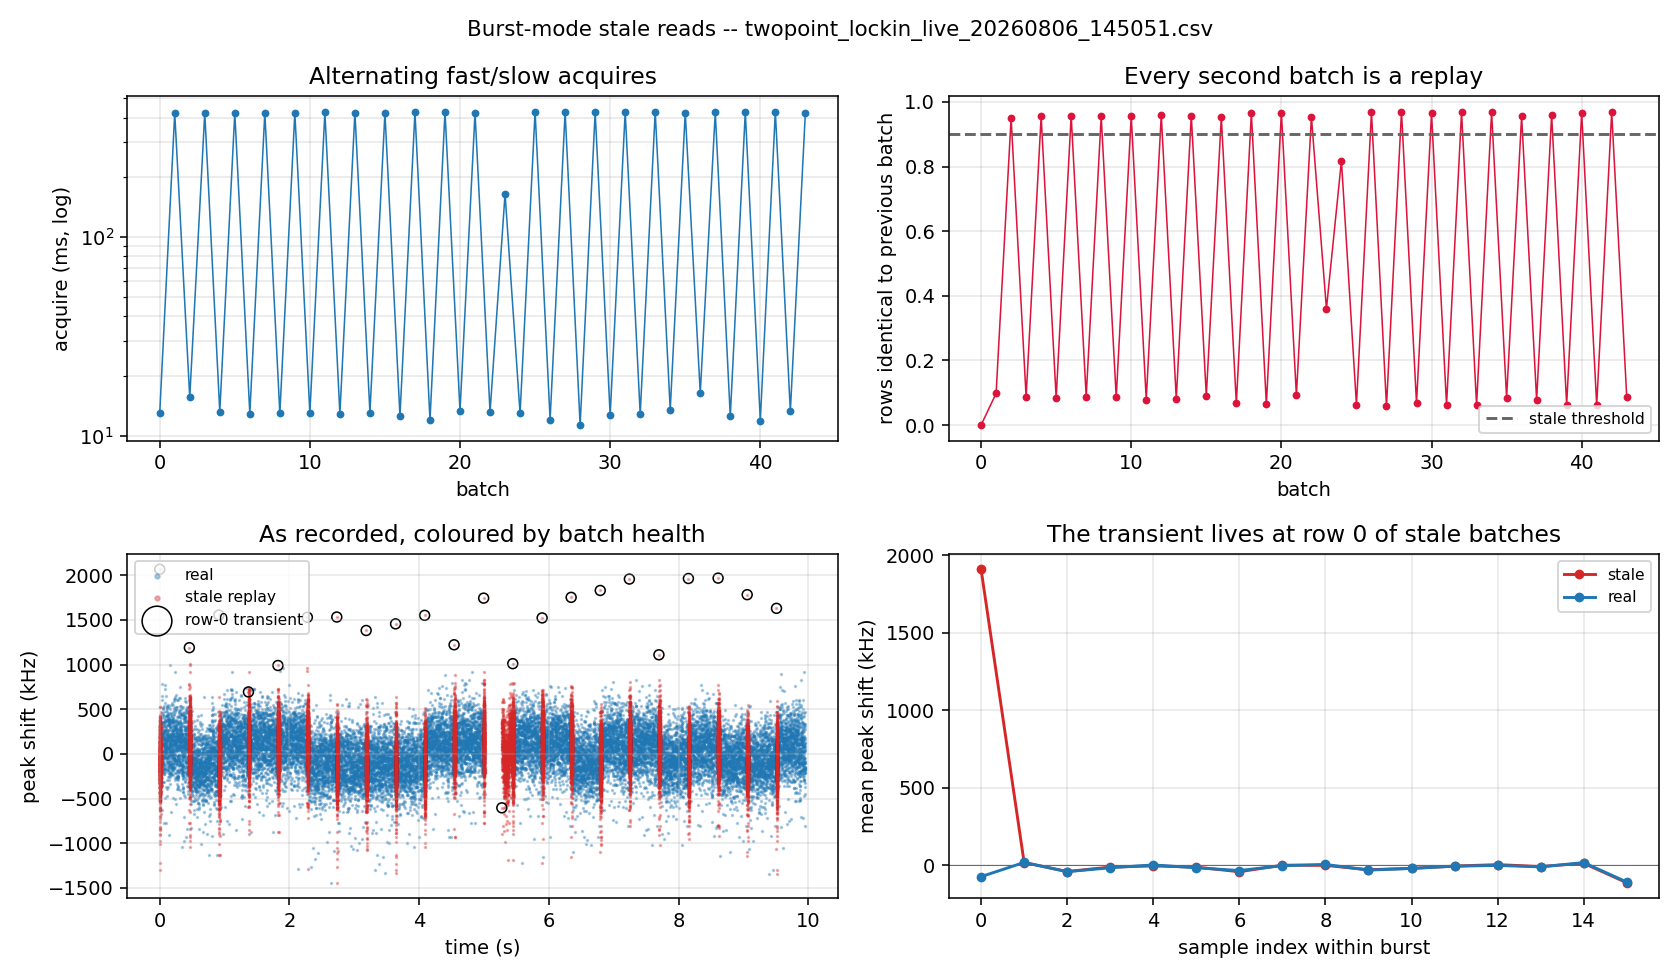
\includegraphics[width=\linewidth]{figures/burst_staleness.png}
\caption{Burst-mode stale reads on 2026-08-06. The stale replays (red) compress
into narrow vertical stripes because their 1000 samples are stamped across a 13\,ms
window while the real samples (blue) spread over 425\,ms. Circled points are the
row-0 transients --- one every $\sim$0.45\,s, exactly the periodicity seen in the
original plot.}
\end{figure}

\section{What to set}

\begin{center}
\small
\begin{tabular}{@{}llp{7.2cm}@{}}
\toprule
\hd{Parameter} & \hd{Recommended} & \hd{Why} \\
\midrule
\co{BURST_ON_STALE} & \co{"drop"} & Re-acquires, then \emph{skips} the batch rather
  than writing a replay to the CSV. Costs duty cycle, not correctness. \\
\co{BURST_STALE_RETRIES} & 2 & The race is transient; a repeat call usually lands
  on a completed run. \\
\co{BURST_REPS} & 500--1000 & See the rate table above; returns flatten past 1000
  and the time-series gaps grow. \\
\co{BURST_DROP_FIRST_REP} & \co{True} & Row 0 runs 1.4\% high --- a real transient. \\
\co{BURST_RESET_TPROC} & \co{True} & Kept available and harmless, but
  \textbf{measured not to fix the replay} (\S\ref{sec:replay}). \\
\bottomrule
\end{tabular}
\end{center}

\section{When to use it}

\textbf{Today, for best sensitivity: this is the mode.} 38\,\etaunit\ at an
effective 3.1\,kHz beats streaming by $\sim$6$\times$ and averaged mode by
7--13$\times$. The price is a 26\% duty cycle loss and a $\sim$15\,ms hole in the
time series every 135\,ms, which matters for a continuous MCG trace and does not
matter for a noise-floor measurement.

If the replay defect is ever fixed, this mode gets $\sim$15\% faster for free. If
the streaming noise defect is fixed, Method C becomes strictly better for
continuous recording.
